\ifdefined\included
\else
\setcounter{chapter}{4} %% Numéro du chapitre précédent ;)
\dominitoc
\faketableofcontents
\fi

\chapter{Interactive Simulator}
\chaptermark{Interactive Simulator}
\label{chap:5}
\minitoc

\section{Introduction}

\section{Interactive Simulator}
planning is same

execution is based on model of execution and mock components

human collaborates in real time with robot in blockwords task

describe simulator, mouse, robot and human capabilities, goal shown, prompt

Synchronization, internal communication through simulated visual signal, explicit reaction time, ID phase currently always successful a success rate can be given. 

*****


In order to simulate collaboration scenarios I developed a dedicated interactive simulator using a Tiago robot. In addition, the automaton described by the MoE has been implemented and integrated with the simulator to provide a proper execution and supervision scheme. Eventually, through carefully designed scenarios and using a shortened version of the PeRDITA questionnaire we gathered the feelings and impressions of the participants regarding the different robot behaviors. We also recorded logs from each executed scenario allowing us to draw a timeline of the execution and compute objective metrics for each scenario among which can be found: the time to complete the task, the human reaction time or the time for the human to be free. Several relevant facts and conclusions can be extracted from the collected results and are discussed in this chapter.

This chapter is organized as follows. First, the interactive simulator functionalities and operations are described. Then the methodology of the user study is provided along with anonymous information on the participants. After, the results obtained are presented and then discussed, validating the proposed hypothesis.


***********

In this section we provide a few functional and technical details about the developed interactive simulator used for the User Study, its overall structure is shown on fig~\ref{fig:simu_architecture}.

\begin{figure}
    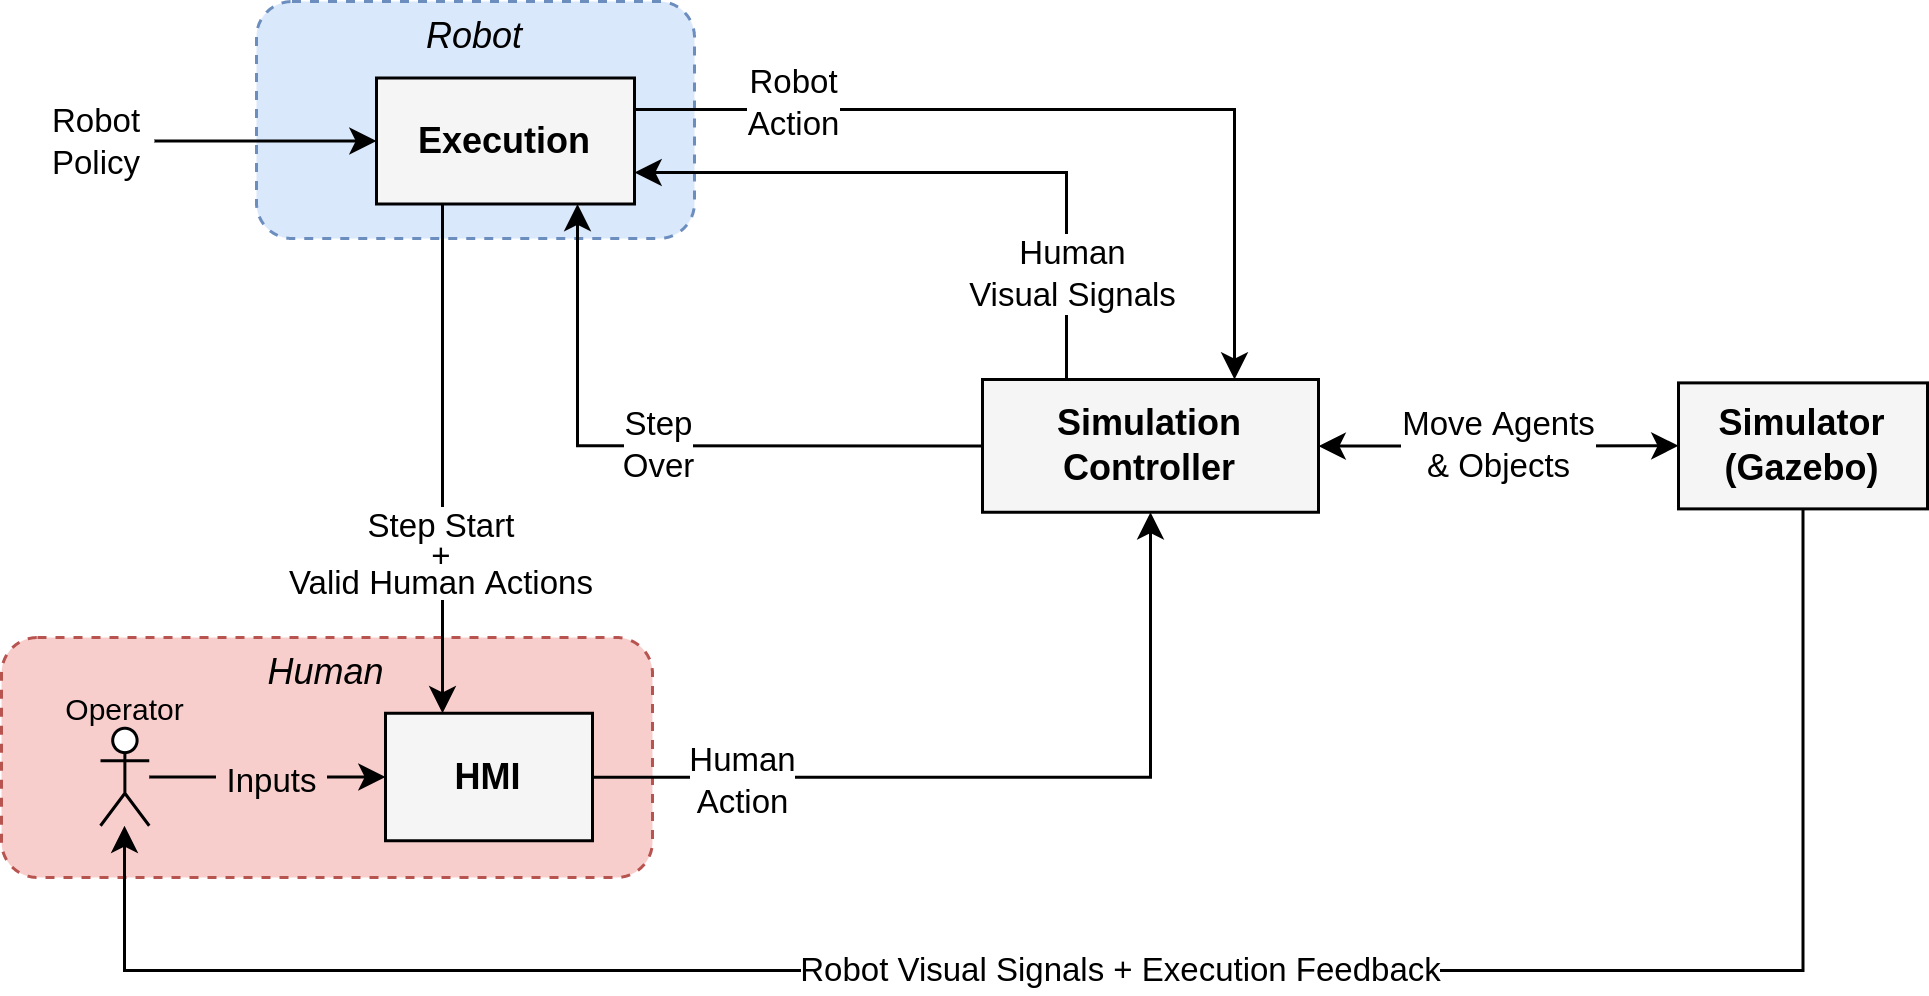
\includegraphics[width=\textwidth]{Chapter6/simu_architecture.png}
    \caption{Overview of the Interactive Simulator's Architecture}
    \label{fig:simu_architecture}
\end{figure}

\begin{figure}
    \centering
    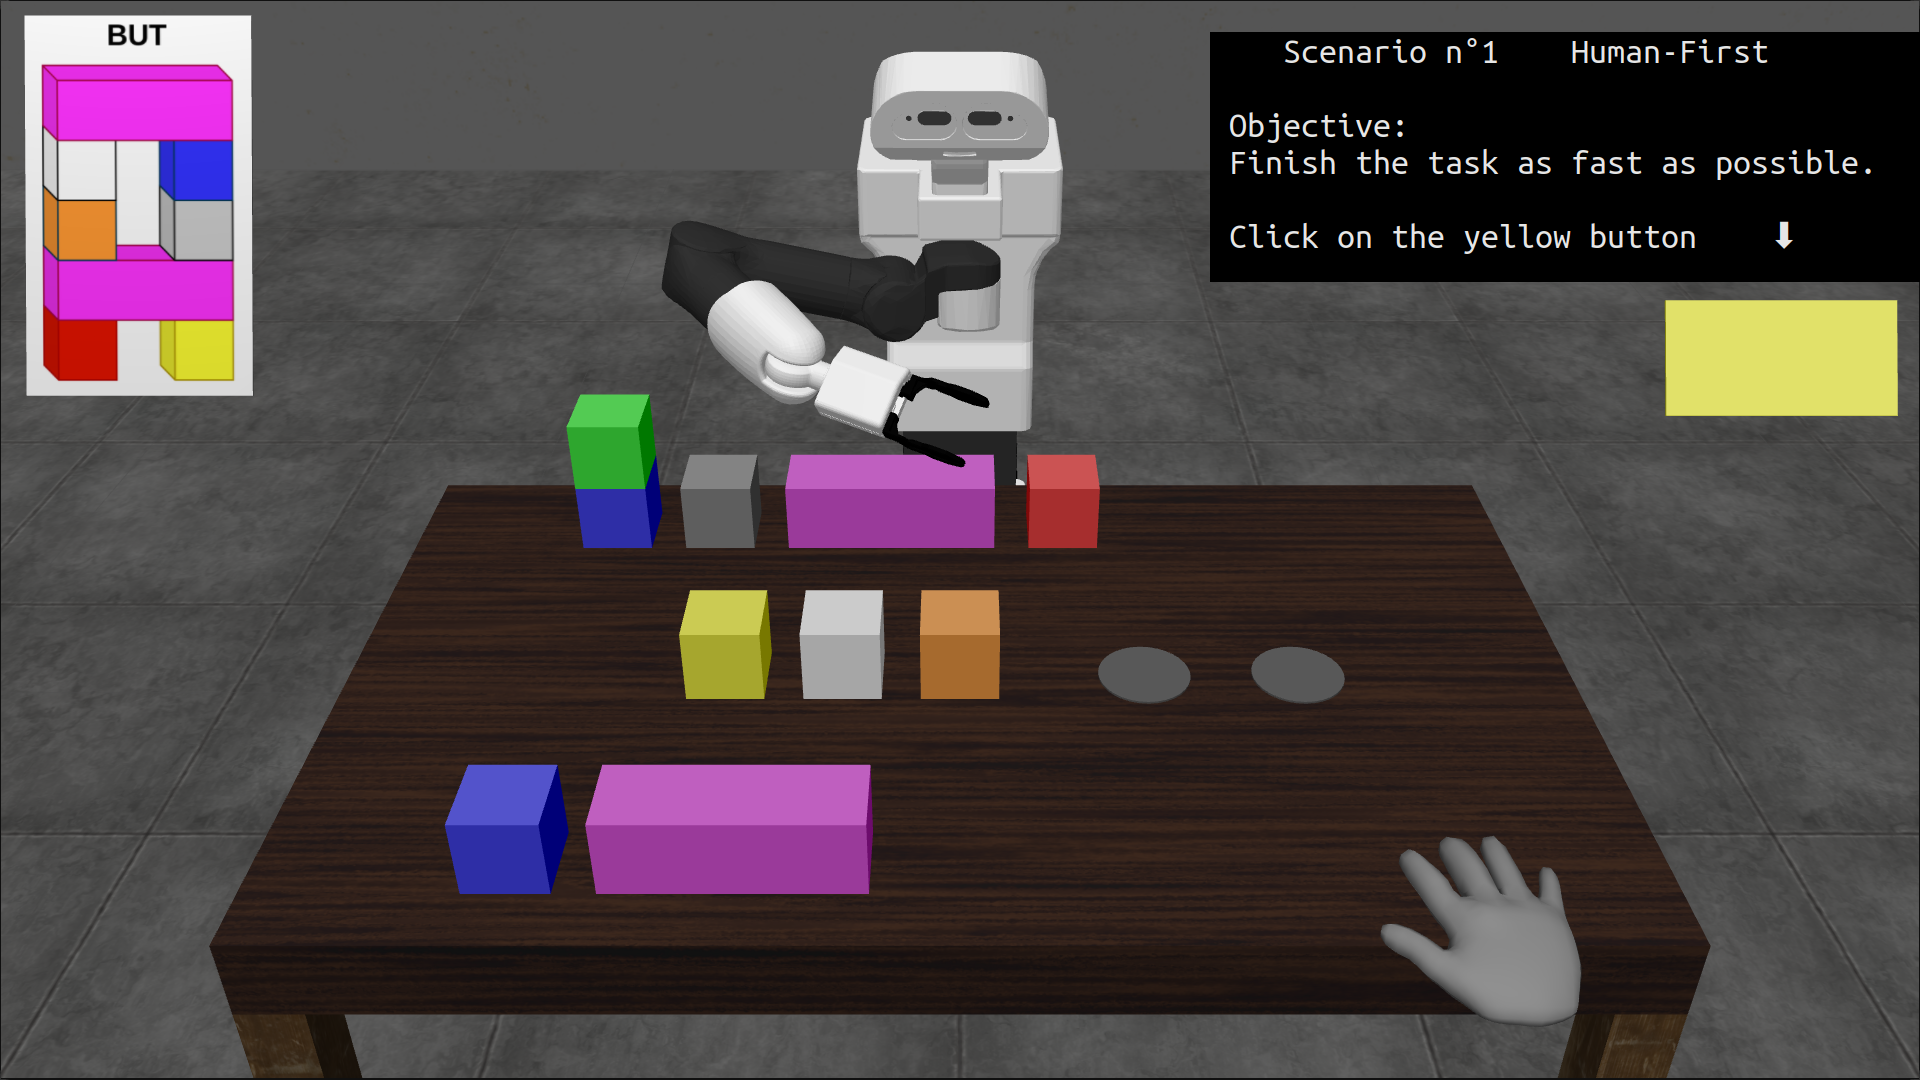
\includegraphics[width=\textwidth]{Chapter6/simu_screenshot.png}
    \caption{Participant view of the interactive simulator. Text prompt. Goal pattern. robot. table. cubes. stacking area. human hand.}
    \label{fig:simu_view}
\end{figure}

First, it is using Gazebo to simulate the scene (table, cubes, agents). 
The robot is a Tiago robot from PAL Robotics. We used a MoveIt controller to plan and execute arm motions. We used a publicly available component to control the gaze of the robot. The head behavior is ad hoc and designed by us.
The human agent is simulated only with its hand which is moved with a handmade dedicated controller. 
For simplicity reasons physics of objects isn't simulated, thus, each agent interact with the scene by statically attaching/detaching object respectively to the robot's gripper or the human hand.
A higher level component called the simulator controller is in charge of translating primitive actions to low level commands and calling the previously presented controllers to make the agent perform actions. Since it manages agent's action, it is also in charge of sending simulated visual signals and indicating when a step is over. Indeed, the agents synchronize themselves using simulated visual signals, and not internal signals. That is, when the human starts performing an action, a brief motion planning phase occur before effectively moving the hand, the motion visual signal is sent to the robot only at this moment. Moreover, to simulate some real perception aspect, a voluntary reaction time is introduced in the robot. Thus, the visual signal can be treated only after this reaction time is passed. A step starts when one agent starts acting (the human or the robot) and it is over when both agents are inactive. Hence, once one agent started to act the other is free to perform an action concurrently and the step will be over only when both are done. If the other agent doesn't act it will be considered as passive/inactive and the step will be over as soon as the first agent finishes.

Then we can find the respective agents' components. The robot component is an implemented version of the model of execution. Its purpose is to supervise the policy execution of the robot while running the automaton described in the model of execution. In practice, the robot starts by indicating when the step started with a sound signal. Then, it waits to receive the visual human signals for a defined amount of time. Without any visual signal the human is considered as passive. The human can either start acting (how will be described just after), which will eventually send a visual signal to the robot, or the human can make an explicit hand gesture to indicate to the robot that they will be passive (this doesn't force the human to be passive for the whole step). Note that even if the robot received the human visual signal of the human starting to act, the actual action being performed isn't yet identified, it only means that the human started to act. The robot must perform a dedicated identification process (ID Phase/Process) to identify the human action. We assume that the hand gesture that the human can make is always successfully identified instantly (without ID Process). Once either the signal received or the time-out reached, if the best robot action doesn't depend on the human decision then the robot can directly start executing this action. The robot action choice is sent to the simulator controller that will start executing the action. If the best robot action depends on the human decision then the human decision must be identified and the ID Process is run. Only after the robot can perform the best action indicated by the policy which is compliant with the identified human action. If the ID Process fails then the robot remains passive, this case is already part of the policy.
Eventually the robot waits for the step over signal from the simulator controller and run the Assessment Process. The latter identify what happened during the step (which action the human performed, even if ID wasn't necessary) and in which state we are to be ready to execute the next step and progress in the policy and toward the goal. 

The human action execution consists in the following. First, the gazebo simulator is made as the main Human-Machine Interface (HMI). Through a handmade plugin one can mouse click in the gazebo simulator window. The click position is sent on a ROS Topic and treated in a dedicated node to potentially trigger a human action. For instance, clicking on a cube starts a "picking" action with the corresponding cube as parameter, clicking on the stack area starts a "place" action, clicking on the table while holding a cube starts a "hold" action, and clicking on the hand make an explicit hand gesture to signal the robot the human desire to be passive. After clicking the hand once, the participant can click another time to indicate the robot full passivity until further notice. The robot will consider the human as unavailable or even not present and will not wait for them. 
For this to be possible we did the following. First, another gazebo plugin has been written to lock the GUI camera as a First Person View and avoid the participant to accidentally move the camera.
Then, at every step, the robot component sends to the component receiving the coordinates of the click the currently valid human actions that the participant can perform. Thus, the participant cannot try to place a cube without holding it. Eventually, each human action is mapped to a clickable zone on the gazebo window. Hence, when the click coordinates are received, we check if it is inside one of the designed zone and is the action associated to the zone is currently valid. If so, then the action decision is sent to the simulator controller to be executed. 
For clarification purpose, when clicking on a cube the robot doesn't immediately know that the human is picking a cube. First, it will know that the human started to act only after receiving the visual signal (after the defined reaction time). And the robot must perform an additional perception phase (ID Process) to identify which action the human performed. 

Additionally, the stacking goal pattern is shown inside the simulator and a small prompt overlay is present to simulate a potential screen with which the robot can communicate its intention to the human during the collaboration. 

Thanks to all these processes, the participant is able to intuitively perform actions using mouse control and can collaborate with the robot to solve the task.

An integrated tutorial has been made to familiarize the participant with the mouse control and the relevant concepts used in the collaboration (notion of step, able to be passive). 
